\documentclass[a4paper,12pt]{article}


\usepackage[english]{babel}
\usepackage[T1]{fontenc}
\usepackage[toc,page]{appendix}
\usepackage{amssymb}
\usepackage{amsmath}
\usepackage{latexsym}
\usepackage{graphicx}
\usepackage{beramono}% monospaced font with bold variant

\usepackage{listings}
\lstdefinelanguage{VHDL}{
	morekeywords={
		library,use,all,entity,is,port,in,out,end,architecture,of,
		begin,and, std_logic_vector, shift_right,signed, end if, end process,if,else,process,not,after,wait
	},
	morecomment=[l]--
}

\usepackage{xcolor}
\colorlet{keyword}{blue!100!black!80}
\colorlet{comment}{green!90!black!90}
\lstdefinestyle{vhdl}{
	language     = VHDL,
	basicstyle   = \ttfamily,
	keywordstyle = \color{keyword}\bfseries,
	commentstyle = \color{comment}
}



\setlength{\parindent}{0pt}
\begin{document}
\section*{MAPD FPGA Lab 5 - Homework Report}
Vincenzo Maria Schimmenti 1204565\\
This homework is about implementing in VHDL a finite impulse response (FIR) filter. A FIR filter is a digital filter characterized by a finite duration impulse response, i.e. calling $c[n]$ the impulse response we would have:
$$c[n]=\begin{cases}
\neq 0 & 0 \leq n \leq N \\
= 0 & \textrm{otherwise}
\end{cases}$$
for some $N \in \mathbb{N}$. Given a signal $x[n]$ the output signal $y[n]$ is the convolution between $x$ and $c$:
$$y[n+1]=c \circledast x = \sum_{i=0}^{N-1} c[i]x[n-i]$$
Our version of the filter employs a filter with five terms. The circuit implementing this FIR filter (also called a 5-tap FIR filter) is shown below:\\
\begin{figure}[h!]
	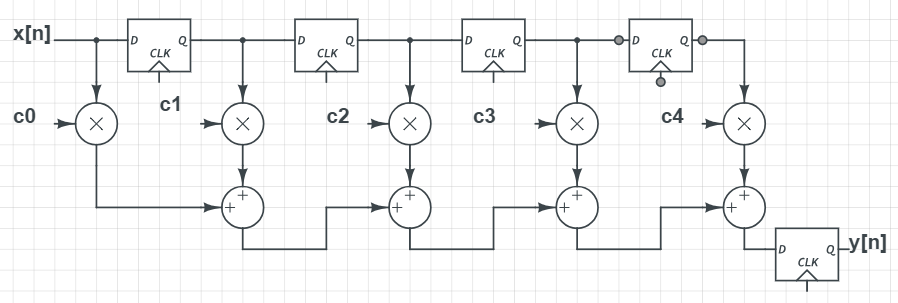
\includegraphics[width=\linewidth]{fir5.png}
	\caption{A 5-tap FIR}
	\label{fig:fir5}
\end{figure}\\
Since the duration of the filter is 5 we need to employ, at each instant $n$, 4 flip-flops to store the previous 4 values of the input and another flip-flop to store the output:
$$y[n+1]=c_0 x[n] + c_1x[n-1]+c_2x[n-2]+c_3x[n-3] + c_4x[n-4]$$
At time $n=0$ all the flip-flops are set to $0$ (thanks to a reset signal). The system is driven by a clock signal that, going from 0 to 1 (the rising edge), triggers the flip flops: at instant $n$, in a parallel fashion, the first flip-flop stores the old input $x[n-1]$ while the other 3 store their left flip flop value; the last flip flop stores the convolution result (and is as well updated by the clock signal).
\newpage For example for $c[0]=1 \quad c[1]=2 \quad c[2]=3 \quad c[3]=4 \quad c[4]=5$ and $x[n]=1 \quad \forall n$ we would get $y[0]=0\quad y[1]=1 \quad y[2] =3 \quad y[3] = 6 \quad y[4] = 10 \quad y[5]=15$. The simulation on Vivado gives:
\begin{figure}[h!]
	\begin{flushleft}
		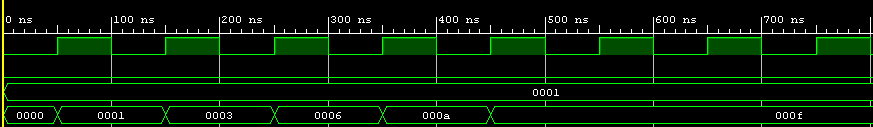
\includegraphics[width=1.2\linewidth,keepaspectratio]{fir5ex.png}
	\end{flushleft}	
	\caption{A 5-tap FIR example: the first row is the clock, the second is the reset signal, the third is the input and the last is the output.}
	\label{fig:fir5ex}
\end{figure}\\
The testbench uses one component, the fir filter component,
which itself uses five flip flop components. All the inputs and outputs are std\_logic\_vectors of length $N=16$ and the operations (addition and multiplication) are done via signed type numbers, either of length 16 or 32. The fir filter entity reads the value from flip flops as logic vectors, converts them into signed, does the convolution then performs the right shift of $Q=11$ bits and takes (since the result of the operation is 32 bits long) the lower 15 bits and the leading sign; in order to do this we used a temporary 32 bit logic vector signal that stores the result of the convolution.
\begin{lstlisting}[style=vhdl]
x_sum_part <=
std_logic_vector(shift_right(c0*signed(x_in)+c1*signed(y01)+
c2*signed(y12)+c3*signed(y23)+c4*signed(y34), Q));

sgn <= x_sum_part(2*N-1);

x_sum <= sgn & x_sum_part(N-2 downto 0);
\end{lstlisting}
(in the code above the $y_{ij}$'s are the values stored in the 4 flip flops and the $c_i$'s, of course, are the filter coefficients)\\
The shift is needed since the coefficents of the filter are supposed to be premultiplied by $2^{11}$ (i.e. left shifted by $11$): this is because we want to use fractional coefficients and in order to do that we need a fixed point representation; our choice is 1 bit for the sign, 4 bits for the integer part and 11 for the fractional part. For example the number $0.19335315$ is in binary represented (approximately) by $0.00110001011$ so the sign bit is $0$ the integer part is $0000$ and the fractional is $00110001011$ so in hexadecimal the number is represented by 0x18B\\
$$0.19335315 \to 0.00110001011 \to 0|0000|00110001011 \to \textrm{0x18B}$$
$$0.20330353 \to 0.00110100000 \to 0|0000|00110100000 \to \textrm{0x1A0}$$
$$0.20668665 \to 0.00110100111 \to 0|0000|00110100111 \to \textrm{0x1A7}$$
As we said the filter's flip flops are driven by a clock signal that we controlled this way:
\begin{lstlisting}[style=vhdl]
fir_clk : process(clk,rst) is
begin
if rst = '1' then
rst <= '0';
else
clk <= not clk after 50 ns;
end if;
end process;
\end{lstlisting}
So if the reset signal is $0$ we set it to $1$ in order to reset all the flip flops (and this happens only once at the start of the simulation) otherwise at each repetition of the process we change the value of the clock (with a period of $50$ ns). After making sure that the FIR was working we used it for the more concrete task of filtering a .wav file; using a python script we created an input file that contained the amplitudes of the .wav file, later passed to a new testbench so it could be filtered. After that we plotted the new spectrum against the filtered one, obtaining:
\begin{figure}[h!]
	\begin{center}
		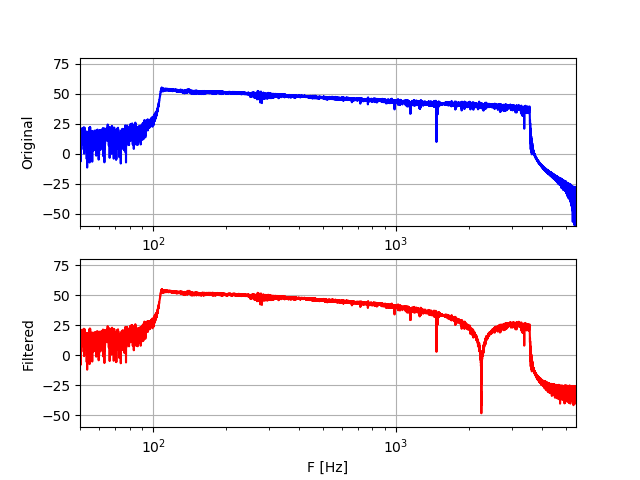
\includegraphics[width=0.6\linewidth,keepaspectratio]{f_spectrum.png}
	\end{center}	
	\caption{The 5 -tap filter applied to a .wav file}
	\label{fig:fir5ex}
\end{figure}
\begin{figure}
	\begin{center}
		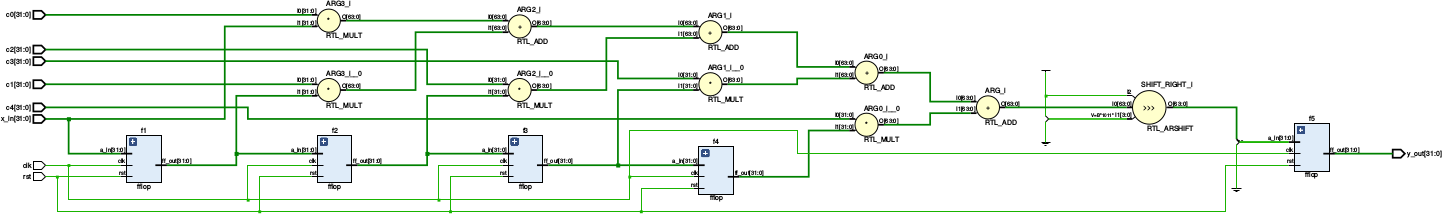
\includegraphics[width=1.7\linewidth,angle=90,origin=c]{schematic.png}
	\end{center}	
	\caption{This is the schematic generated by Vivado for the FIR filter}
	\label{fig:schematic}
\end{figure}
\end{document}